\chapter{Technology Overview}
\label{section:theory}

This chapter provides a brief overview over the technologies that will be used in this thesis.


\section{Accelerator Architectures}


Since the release of NVIDIA CUDA general purpose computing on graphics processors has become mainstream.
In recent years, FPGA vendors Altera and Xilinx are pushing into the HPC field as well.
This section describes the architectures of these two accelerators.



\subsection{Graphics Processors}

Graphics processing units (GPUs) were originally developed for graphics and visualization applications.
As such, they are designed to handle mounds of data like vertices or pixels in a short amount of time.
These capabilities are also useful for other types of data.
For this reason, GPUs are today used also for high performance general purpose computing, known as \emph{GPGPU}.



GPUs differ from traditional general purpose processors (CPUs) primarily through a much higher degree of parallelism.
CPUs are built to be easy to use and versatile, being able to handle many different tasks. Graphics processors in contrast, are meant to deal with large amounts of data as fast as possible. Around 1998 the number of transistors on GPUs overtook that of CPUs because most of the die area for CPUs is dedicated to cache and control logic, whereas the die area of GPUs is mostly dedicated to computational logic, thus providing more computing power \cite{wilt}.
Additionally this makes them more energy efficient, offering more performance per Watt.
As an example, a modern GPU like the GK110 class from NVIDIA (released 2012) features 7.1 billion transistors \cite{gk110}.


%in the beginning only single precision floating point

The disadvantages of GPUs include a more demanding programming model because of comparatively little die area dedicated to control logic.
Optimally, the task should be \emph{embarrassingly parallel} and require little synchronization.
NVIDIA graphics cards can be programmed with the CUDA \cite{cudaguide} or OpenCL \cite{opencl} platforms.

For high performance computing, graphics processors are typically used as accelerators in conjunction with a host CPU system where the main application is running.
This adds the drawback of communication delay between the host and the GPU which very often constitutes a bottleneck for an application.

%TODO:
%cuda, gpgpu
%power-wall
%multicore: more generic
%pros & cons table?
%SIMD!


In the following paragraphs, a brief overview of the GPU architecture using the example of the NVIDIA Kepler (GK110) class is provided. Other GPU architectures, also from other vendors, are organized in a similar fashion.


The GK110 employs a deep hierarchy of components. 
Up to 15 \emph{Streaming Multiprocessors} (SMX) constitute the centerpiece of the GK110. Each of the SMX units consists of 192 \emph{CUDA cores}.
Each CUDA core in turn is composed of a floating point unit and an integer arithmetic logic unit. The cores are pipe-lined and can execute one operation per clock cycle.
In addition to CUDA cores, each SMX also contains 64 double-precision floating point units (DPU), 32 load/store units for the computation of source and destination memory addresses and 32 special function units (SFUs) for fast approximations of transcendental operations such as sine, square root or interpolation.
A SMX organizes the instruction execution in groups of 32 threads (\emph{warps}). 4 \emph{warp schedulers} per SMX can issue 2 instructions to a warp in each clock cycle, theoretically utilizing all cores to full capacity. \cite{gk110} 

A 256KB large register file per SMX provides 256 32-bit registers for each CUDA core and DPU. Each SMX employs additional 16 texture filtering units, 48KB read-only data cache and 64KB memory that can be split up in either L1 cache or shared memory for communication between threads.
The 1.5MB L2 cache can be accessed by all SMX units. Finally 6 memory controllers for GDDR6 DRAM complement the memory hierarchy. \cite{gk110} 

For the communication with the host, typically the PCIe bus is used. Chapter \ref{pcie} provides a brief overview over this protocol.


%TODO: programming: (glsl), cuda, opencl



\begin{figure}[htb]
	  \centerline{
		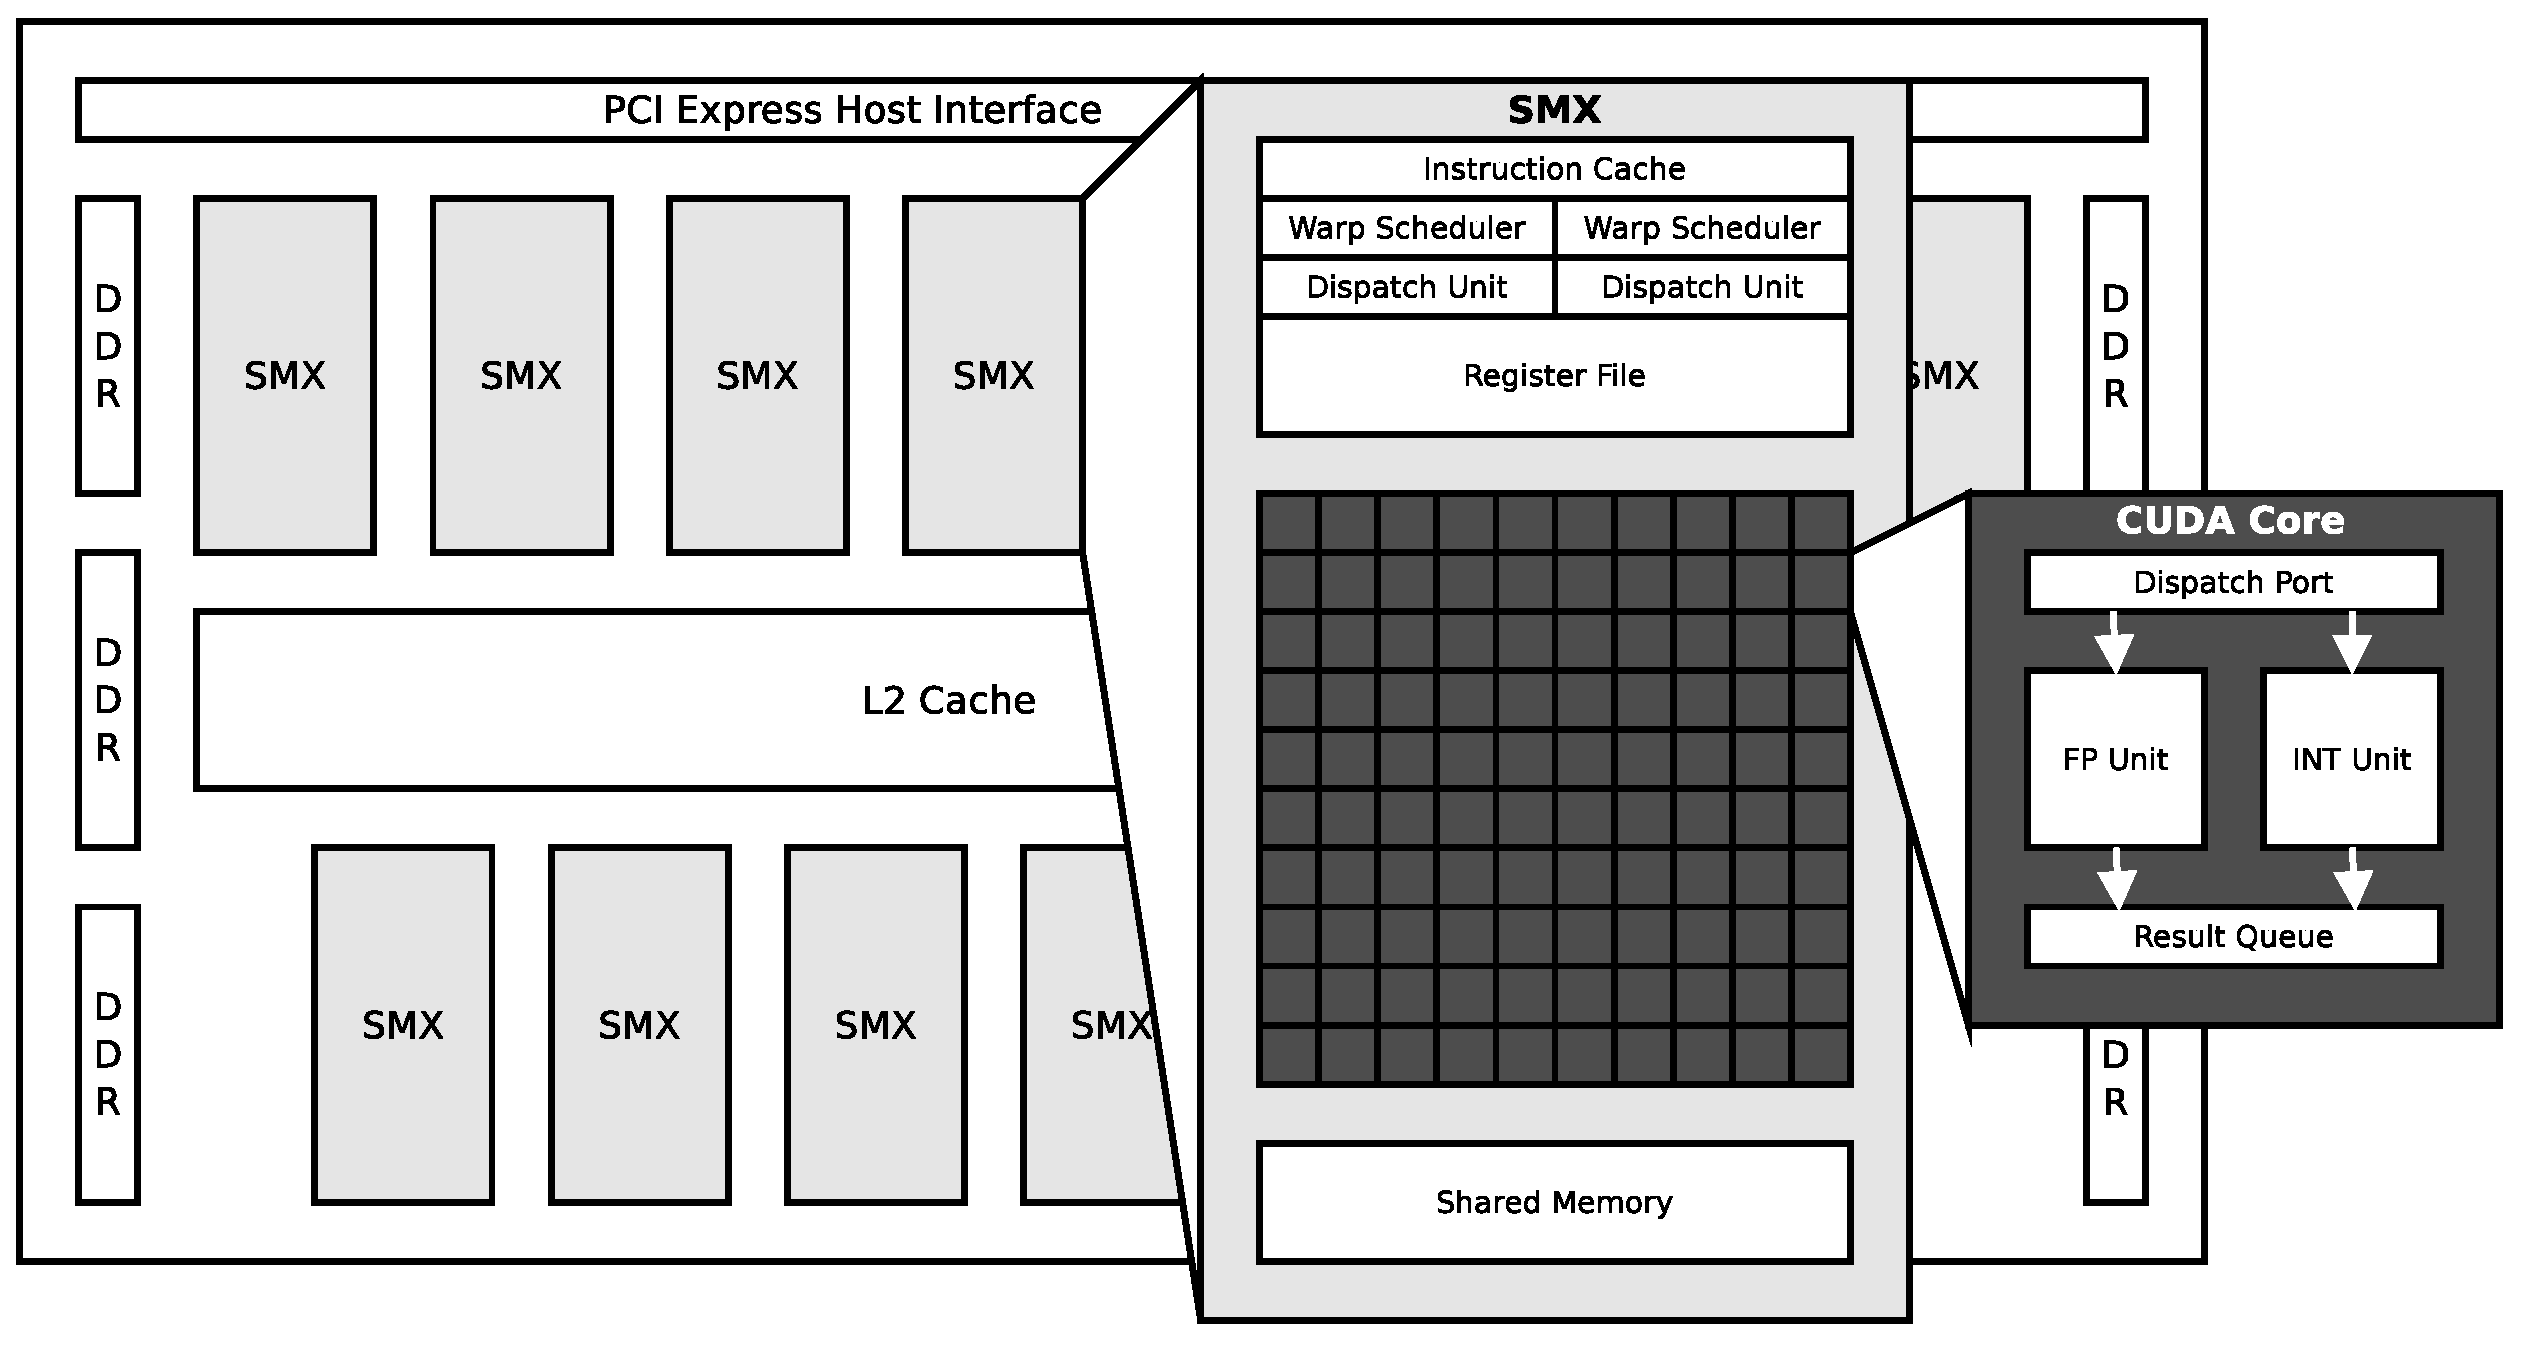
\includegraphics[width=1.0\textwidth]{images/gpuarch.eps}}
	  \caption{Simplified schematic diagram of the NVIDIA GK110 class GPU architecture. (Image based on \cite{gk110})}
	  \label{fig:gpuarch}
\end{figure}









\subsection{Field Programmable Gate Arrays}


%fundamentally different from cpus and gpus
%architecture (seminar)
%altera opencl
%board layout? dram,fpga chip, pci

\emph{Field Programmable Gate Arrays} (FPGAs) are fundamentally different from CPUs and GPUs.
In contrast to processors, FPGAs are not programmed by specifying a list of sequential instructions to execute, but by constructing digital electronic circuits.
These circuits can execute in parallel and do not have the overhead of instruction
fetching and decoding.
This can result in hundreds of times faster performance in addition to lower power consumption compared to software-based designs \cite{hauck}.


Very generally speaking FPGAs consist of a large number of \emph{look-up tables} (LUTs) that can be connected together to implement any digital circuit.
A LUT is a block of memory that stores a small number of bits.
It can be implemented with SRAM cells and multiplexers that select which cell to route to the output.
An arbitrary Boolean function can be implemented by storing the truth table of the function in the SRAM cells \cite{hauck}. Figure \ref{fig:LUT} shows an example LUT that implements the 3-input XOR function or a 1-bit full adder.


\begin{figure}[htb]
	  \centerline{
		\includegraphics[width=1.0\textwidth]{images/LUT2.png}}
	  \caption{Left: A look-up table loaded with the values of the 3-input XOR function which can also be seen as a 1-bit full adder without the carry output (Image based on \cite{farooq}). 
	  Center: A truth table describing
the same function. 
	Right: An equivalent digital circuit consisting of logic gates.}
	  \label{fig:LUT}
\end{figure}

More complex functions can be achieved by combining multiple look-up tables.
For example the addition of two 8-bit unsigned integers can be implemented using 8 1-bit full adders from figure \ref{fig:LUT} and 8 LUTs storing the carry logic.
They are then connected as shown in figure \ref{fig:ripple}.
Actually, this design can be optimized to use less LUTs.


\begin{figure}[htb]
	  \centerline{
		\includegraphics[width=0.65\textwidth]{images/rippleadder.png}}
	  \caption{A ripple-carry adder implemented using only 3-input LUTs}
	  \label{fig:ripple}
\end{figure}

%TODO size of LUTs

Look-up tables can only act as logic functions, not able to store a state.
Therefore LUTs are connected to a \emph{D-type flip-flop} which acts as an output buffer.
Together they form a \emph{logic block} or \emph{cell}.
A multiplexer selects whether the logic block's output comes from the LUT directly or from the flip-flop.
The multiplexer in turn is configured by an additional SRAM cell \cite{farooq}.
In reality logic blocks often include additional components such as carry logic or full adders because they are often used \cite{altera_arch}.

%TODO: altera/xilinx logic block diagram

A logic block on its own can only perform very simple logic functions. For more complicated computations the
cells have to be connected together.
Usually, these interconnections constitute up to 90\% of the whole FPGA’s area \cite{farooq}.
This is required for a high degree of flexibility to be able to implement any digital circuit.
The most common architecture is the \emph{island style} interconnect \cite{hauck} which is outlined in figure \ref{fig:island}.
Instead of connecting the logic blocks directly with each other, they are separated by horizontal and vertical multi-lane signal channels.
On intersections configurable \emph{switch boxes} control which direction a signal takes.
The logic blocks are connected via \emph{connection blocks} to the channels.
Again, connection blocks can also be configured to allow to connect any lane to the cell’s input or output.
To also improve the signal delay from one logic block to another, additional long-distance lanes in the channels can be used.
Most commercial FPGAs (e.g. Altera Stratix and Xilinx Virtex families \cite{altera_arch}) employ this concept as the basis for their routing architectures.


\begin{figure}[htb]
	  \centerline{
		\includegraphics[width=0.85\textwidth]{images/island_style.png}}
	  \caption{Example of an island style connectivity (Components are not to scale. Image based on \cite{hauck}}
	  \label{fig:island}
\end{figure}


In theory a FPGA can consist only of configurable logic blocks, interconnections and I/O pins.
However, to achieve higher performance vendors usually employ dedicated non-configurable (\emph{hardened}) hardware for often used and expensive operations. 
For instance, multipliers, DSP blocks and dedicated SRAM cells, distributed across the chip are very common in modern FPGAs.
Moreover some models may include complete hard CPUs for computations that are inherently sequential or to run a whole operating system.
Altera’s Cyclone V SoC series for example includes an ARM Cortex-A9 core \cite{altera_arch}.


In contrast to compiling a software program, FPGA configuration is not a straight-forward process, as outlined in figure \ref{fig:configflow}.
For one, yielding decent results almost always requires optimization towards one of two often contradicting goals: minimal resource usage vs. performance.
Furthermore, after each step several constraints have to be met, most important
one being that the design does not require more resources than are available on the target chip.
If one of those constraints cannot be maintained the procedure needs to be restarted with a different optimization strategy.
This contributes to rather long build process.


\begin{figure}[htb]
	  \centerline{
		\includegraphics[width=0.40\textwidth]{images/configflow.png}}
	  \caption{The major phases involved in the configuration procedure. Falling back to a previous step may be required if a constraint cannot be met. (Image based on \cite{hauck})}
	  \label{fig:configflow}
\end{figure}

The most commonly applied method to configure FPGAs is to use a \emph{hardware description language} (HDL) such as \emph{VHDL} or \emph{Verilog}.
HDLs differ fundamentally from imperative programming languages like C or Fortran because of their concurrent semantics \cite{hauck}.
A logic synthesizer converts the HDL code into a set of primitives, called a \emph{netlist} which basically consists of logic gates, flipflops and the interconnections between them.
These netlist primitives are then mapped to the target device's primitives (i.e. LUTs of certain sizes, various DSP units).
Next, every element of the new technology-mapped netlist is assigned to a real physical building block of the corresponding type on the chip and a the connections between them are established.
In the end, if the timing simulation satisfies the target clock rate, a bitstream containing the contents of the memory cells of the LUTs, multiplexers and switches is produced.

HDLs provide a great flexibility and the ability to control the flow of every digital signal in every clock cycle.
However, this demands a high level of expertise and long development time.
In 2013, Altera released an SDK for the configuration of their FPGAs with the OpenCL standard \cite{altera_opencl}.
This enables to program FPGAs in the same way as GPUs.
This standard is described in more detail in section \ref{section:opencl}.

It is difficult to compare the performance of FPGAs to GPUs because of the completely different architectures.
Very generally speaking, FPGAs are better suited for integer operations, GPUs on the other hand achieve better results with floating point calculations.
Moreover, FPGAs are very flexible and can interface a variety of other devices \cite{chimera}.


%TODO: 
%altera opencl
%lower power consumption / high purchasing cost
%benchmark comparisons? "It is difficult to compare the performance of GPUs to FPGAs"
%extremely flexible at interfacing other devices



\section{OpenCL}
\label{section:opencl}


\emph{OpenCL (Open Computing Language)}\cite{opencl} is a standard for heterogeneous high performance computing managed by the Khronos consortium.
It has been implemented on a wide range of devices, most importantly multi-core CPUs, GPUs and FPGAs.
It defines a high level abstraction layer for low level hardware instructions.
This enables to scale computations from general purpose processors to massively parallel devices without changing the source code.




The OpenCL specification resembles in many aspects the NVIDIA CUDA platform and can be roughly summarized as follows\cite{opencl}:

An OpenCL application runs on a \emph{host} system which is connected to one or more accelerator \emph{devices}.
A device, divided into \emph{compute units} and \emph{processing elements}, is usually able to execute compute \emph{kernels} in a SIMD or sometimes SPMD fashion.
The kernels are mostly written in the \emph{OpenCL C} programming language, a dialect of the C99 standard and compiled with a vendor-specific compiler, but native kernels are optionally supported as well.
They describe the sequence of instructions within a single execution instance, called a \emph{work-item}.
Work-items that are grouped in the same \emph{work-group} are executed concurrently.


The memory hierarchy consists of four distinct regions for the kernels:
\begin{itemize}
	\item \emph{Global} memory that can be written and read by all work-items in all work-groups
	\item \emph{Constant} memory, a region of global memory that is initialized by the host and does not change during the execution
	\item \emph{Local} memory that is only accessible to work-items within the same work-group
	\item \emph{Private} memory owned by a single work-item and not visible by others
\end{itemize}

The functions \texttt{clEnqueueWriteBuffer} and \texttt{clEnqueueReadBuffer} provide a convenient way to transfer data between host and device memory.
Methods for data transfers between multiple devices are not specified by the standard.
This is only possible with vendor-specific extensions.
Specifically for GPU-FPGA transfers, no extensions are available.
The only portable workaround is to read a memory region from the first device into CPU memory and then write it to the second device.
Obviously, this approach is rather slow, due to the overhead of the two transfers.




The \texttt{cl\_khr\_icd} extension\cite{icd} allows multiple OpenCL implementations from different vendors to co-exist on the same system.
It defines an \emph{installable client driver (ICD) loader}, a unifying library that acts as a mediator between the different platforms.
This enables the use of multiple heterogeneous devices in a single process without the different implementations interfering with each other.
Without this mechanism, the overhead of multiple processes and inter-process communication (IPC) inbetween them is required.
As of the time of this writing, Altera's latest SDK version 14.1 does not support this extension yet.
Section \ref{section:icd} describes an implementation of an incomplete yet usable ICD for Altera OpenCL.



%TODO:
%example data transfer?
%synchronization?
%command queues
%




\section{Linux Device Drivers}
\label{section:drivers}

Hardly any two hardware devices provide the same control interface to the host system.
As a consequence either an application program has to know how to interface every single device (which is impossible for those that are not yet available)
or an abstraction layer between the application software and the actual device is needed.
The role of a \emph{device driver} is to provide this abstraction layer \cite{ldd}.
A driver is built for a specific piece of hardware and knows its internal logic.
The user program may use a set of standardized calls that are independent of the hardware and the device driver will map these calls to the hardware specific commands.


A device driver communicates with the peripheral device through its I/O registers.
Using hardware registers is very similar to main memory: 
Every register has an address which can be accessed with the \texttt{read} and \texttt{write} system calls.
The CPU is then asserting electrical signals on the address bus and control bus and  reading from or writing to the data bus \cite{ldd}.
The most important difference is that I/O regions can and do have side effects whereas memory usually does not.


Direct I/O access to a hardware device may cause physical damage if operated incorrectly. Therefore in Linux, this is only allowed for the privileged code running in kernel space.
Though the Linux kernel is largely monolithic, it allows \emph{modules} to be built separately from the rest of the kernel and inserted or removed at runtime when needed, without having to reboot the whole system.
Device drivers are usually constructed as kernel modules \cite{ldd}.

A kernel module does not have a \texttt{main} function and is completely event-driven \cite{ldd}.
It has to provide an initialization function which may initialize the hardware and register callbacks for hardware interrupts or user space communication calls.
A minimal kernel module written in C looks like this:
\begin{lstlisting}[label=some-code,caption=Minimal kernel module]
#include <linux/init.h>
#include <linux/module.h>

static int hello_init(void)
{ printk(KERN_ALERT "Hello, world\n"); return 0; }

static void hello_exit(void)
{ printk(KERN_ALERT "Goodbye\n"); }

module_init(hello_init);
module_exit(hello_exit);
\end{lstlisting}

To insert a module into the kernel at runtime, the following command can be used:
\begin{lstlisting}
	insmod path/to/example_module.ko
\end{lstlisting}

The following command will remove the module from the kernel again:
\begin{lstlisting}
	rmmod example_module
\end{lstlisting}

In Linux, the main method for a user space program to communicate with a kernel module is through file operations on a file exposed by the module.
Such a \emph{device file} is usually located in the \texttt{/dev/} directory of the file system.
The module can register callback functions that are executed when system calls like \texttt{open}, \texttt{read} or \texttt{ioctl} are performed on this file.



Both, Altera and NVIDIA provide Linux drivers for their chips.
Altera released its PCIe driver under an open source license, available for modification, whereas the NVIDIA driver is split into two parts: the kernel module which is also open source and the actual closed source driver. The kernel module acts only as an mediator between the user programs and the actual driver.

%TODO:
%printk, dmesg, /var/log?
%actual hardware I/O
%interrupts
%nvidia & altera examples? nouveau?

\section{PCIe}
\label{pcie}

\emph{Peripheral Component Interconnect Express} (PCIe) is a very commonly used bus for the connection of peripheral devices to a host system.
It is an extension of the PCI bus and is completely compatible with its predecessor up to the point that PCI-only devices can communicate over PCIe without modifications \cite{pcie}.

A PCIe interconnect that connects two devices together is referred to as a \emph{link}.
A link consists of either x1, x2, x4, x8, x12, x16 or x32 signal pairs in each direction, called \emph{lanes}. Data can be transmitted in both directions simultaneously on a transmit and receive lane.
The signal pairs are \emph{differential}, that means that 2 electrical signals with opposing voltages (\texttt{D+} and \texttt{D-}) are used for each logical signal.
A positive voltage difference between \texttt{D+} and \texttt{D-} implies a logical \texttt{1} and logical \texttt{0} for a negative difference.
Differential signals have the advantage that they are more robust towards electrical noise.
Each PCIe lane thus totals to overall 4 electrical signals. \cite{pcie}

The PCI Express 2.0 specification supports 5.0 Gbits/second/lane/direction transfer rate. %TODO cite pcie specs?
For an additional degree of robustness during data transfer, each byte of data transmitted is converted into a 10-bit code (\emph{8b/10b encoding}) i.e. for every byte of data, 10-bits are actually transmitted, resulting in 25\% overhead.
The 8b/10b encoding moreover guarantees one-zero transitions in every symbol, which eliminates the need of a clock signal.
The receiving device can recover the sender's clock through a \emph{PLL} from the rising and falling edges of the signal \cite{pcie}.
The following table shows the maximum possible transfer speeds with PCIe:


\begin{center}
\begin{tabular}{| l | c |}
	\hline
	PCIe link width & Theoretical bandwidth in one direction\\
	\hline
	x1 &   500 MBytes/second\\
	x8 &   4   GBytes/second\\
	x32 &  16   GBytes/second\\
	\hline  
\end{tabular}
\end{center}

The PCI Express hierarchy centers around a \emph{root complex}. It connects the CPU and the memory subsystem to the PCIe fabric consisting of endpoints and \emph{switches} which may extend the hierarchy.
Its functionality includes the generation of transactions on the behalf of the CPU and routing of packets from one of its ports to another. \cite{pcie}
An example topology is illustrated in figure \ref{fig:pcie_topo}.

%TODO: diagram
\begin{figure}[htb]
	  \centerline{
		\includegraphics[width=0.7\textwidth]{images/PCIE.eps}}
	  \caption{Example topology of a system employing PCIe (Image based on \cite{pcie})}
	  \label{fig:pcie_topo}
\end{figure}


In PCI Express data is transferred from one device to another via \emph{transactions}.
A transaction is a series of one or more \emph{packets} required to complete an information transfer between a sender and a receiver. \cite{pcie}
Transactions can be divided into 4 address spaces:
\begin{itemize}
	\item \emph{Memory}: Data transfer to or from a location to the system memory or a device.
	\item \emph{IO}: Data transfer to or from a location to the system IO map. PCIe devices do not initiate IO transactions. They are intended for legacy support.
	\item \emph{Configuration}: Read from or write into the configuration space of a PCIe device. Only initiated by the host.
	\item \emph{Message}: General messaging and event reporting
\end{itemize}



The \emph{configuration space} of a device contains a set of standardized registers used by the host to discover the existence of a device function and to configure it for normal operation.
A device may implement multiple functions.
Each function's configuration space is 4KB large of which the first 256 Bytes are occupied by the legacy PCI header.
This header includes the \emph{Vendor ID} and \emph{Device ID} registers to identify a device, \emph{Status} and \emph{Command} registers used to report and control certain features of the device as well as up to 6 32-bit \emph{Base Address Registers (BARs)}. \cite{pcie} 
Two BARs can be merged into one 64-bit BAR.
A device may expose a linear window of its memory into one of the BARs.
The host or another PCIe device may then use the value programmed into the BAR as a physical address to write from or read into the device's memory in the same way as to system memory, i.e. via Memory Read or Write Transactions. \cite{rdma}
%TODO diagram/table of the header?
%diagram from rdma page?



%interrupts
A PCI Express device may deliver interrupts to its device driver on the host via \emph{Message Signaled Interrupts (MSI)} \cite{pcie}.
A MSI is a Memory Write transaction to a specific address of the system memory which is reserved for interrupt delivery.
Moreover legacy interrupts employing dedicated physical pins are supported. Interrupts are useful for a high degree of performance.
Instead of the host polling the state of a device, the device can notify the host when an event, such as a completed data transfer, occurs.

%hardware specs
%form factor image?
%bus mastering


\section{Direct Memory Access}

\emph{Direct Memory Access} (DMA) is a hardware mechanism that allows peripheral components to transfer data directly to and from main memory without involving the system processor \cite{ldd}.
DMA is useful when the CPU is not able to keep up with the transfer rate or has to perform other operations inbetween. This can increase not only the throughput to and from a device but also the overall system performance.

DMA is carried out by a \emph{DMA controller} built into the device.
DMA transfers can be classified as \emph{synchronous} or \emph{asynchronous}. 
In the asynchronous case the device initiates the accesses to the system memory.
This is mostly done by acquisition devices or network cards.
A synchronous transfer is initiated by the software and contains roughly the following steps \cite{ldd}:
\begin{enumerate}
	\item The driver sends a command to the device's DMA controller containing the memory address to read from or to write into. The associated process is put to sleep so that the CPU can process other tasks.
	\item The DMA controller performs the transfer and sends an interrupt to the driver when it is completed.
	\item The interrupt handler acknowledges the interrupt and wakes up the process.
\end{enumerate}


%virtual/physical/bus address space
It is important to note that a DMA controller requires an address from the \emph{bus address space} whereas whereas software operates on the \emph{virtual address space}.
The virtual address space is managed by the operating system and the \emph{memory management unit (MMU)}, a hardware component usually built into the processor chip \cite{tanenbaum}.
The virtual address space is segmented into \emph{pages} of equal size\footnote{in Linux by default 4KB}.
A \emph{page table} on the MMU maps from pages to the real physical memory.
Every process gets a set of pages assigned by the OS.
When a process needs to access the main memory, the CPU sends the virtual address to the MMU, which translates it through the page table to the actual \emph{physical address} of the system memory.
In case there is no page table entry for the specified virtual address a \emph{page fault} exception is signaled to the OS.
This can happen due to the software accessing a memory area it is not allowed to or if the memory is full and the requested page has been moved from the RAM to the swap partition on the hard drive.
In the latter case the OS loads it from the swap and puts it back to the RAM, replacing another page.


This mechanism frees programs from the need to manage shared memory, allows processes to use more memory than might be physically available and increases the security by disallowing a process to access memory outside of its address space \cite{tanenbaum}.



Bus addresses are used between a peripheral bus and the system memory.
An \emph{I/O memory management unit (IOMMU)} may play the same role as the MMU and translate from the bus address space to the physical address space.
However, often the IOMMU is not present in the system or deactivated, in which case the bus addresses are equivalent to physical addresses \cite{ldd}.
This scenario is assumed throughout the rest of this thesis as it represents a majority of today's systems and for the sake of convenience.
Figure \ref{fig:address_spaces} illustrates the relations between the address spaces.


\begin{figure}[htb]
	  \centerline{
		\includegraphics[width=1.1\textwidth]{images/address_spaces.eps}}
	  \caption{Relationship between the different address spaces with example mappings. In this case the IOMMU performs a 1:1 mapping. (Image based on \cite{tanenbaum,ldd})}
	  \label{fig:address_spaces}
\end{figure}



Physical addresses are usually not visible neither to the user application nor to the driver.
To get the physical address of a buffer that was allocated in user space, an operation called \emph{pinning} is required \cite{ldd}.
Pinning marks pages as not swappable to ensure that they are not moved out to the swap partition.
This ensures that the virtual address of the page always maps to the same physical address.
The \texttt{get\_user\_pages(...)} function can be used within the driver to perform this operation.
It also provides the physical addresses to each page it pins.

%scatter-gather
Unfortunately, especially for large buffers, the acquired physical addresses do not form a contiguous block, but are distributed across the memory.
A DMA controller that supports \emph{scatter-gather} operations can accept a scatter-list, an array of addresses and lengths, and transfer them in one DMA operation \cite{ldd}.
For controllers that to not support this feature, either a contiguous buffer has to be allocated (for the write direction) or multiple transfers are required.

DMA is indispensable in the HPC field and most accelerator cards have a built-in DMA controller.
For example in Altera OpenCL a modular Scatter-Gather-DMA (SGDMA) IP core \cite{altera_ip} is used for transfers of at least 1KB size.

Starting with the Kepler class architecture, all NVIDIA Quadro and Tesla cards additionally employ a technology called \emph{GPUDirect RDMA} \cite{rdma}.
With RDMA, the GPU is able to pin a buffer in its internal memory and expose it into one of the PCIe BARs.
This BAR can be used as a bus address for other devices within the bus to directly write into or read from the GPU memory without the overhead of transferring the data to system memory first.


%TODO
%burst mode?
%cycle stealing mode?
%transparent mode?

%cache coherence

%GPUdirect rdma inkl virtual gpu address space

%example: dma controller on the altera fpga





















%\section{Previous Work} % TODO: own chapter?
\chapter{Previous Work}
\label{section:previouswork}


Parts of the issues addressed in this thesis have already been tackled in the past.
This chapter gives a brief overview of the previous research.
A detailed comparison of this thesis and these other approaches is presented in section \ref{section:previousworkcomparison}.



\section{Ray Bittner \& Erik Ruf}
\label{bittner}

Ray Bittner and Erik Ruf from Microsoft Research implement direct GPU-FPGA communication with a custom IP core, named \emph{Speedy PCIe} \cite{bittner,bittner_speedy}.
The IP is written for Xilinx FPGAs and designed to exploit the full bandwidth potential of the PCIe bus.
A Microsoft Windows driver is also supplied for the core.

\begin{figure}[htb]
	  \centerline{
		\includegraphics[width=0.6\textwidth]{images/speedypcie.png}}
	  \caption{Speedy PCIe IP core design (Image from \cite{bittner_speedy})}
	  \label{fig:speedypcie}
\end{figure}


Bittner and Ruf discovered that several CUDA operations that are intended for GPU-CPU data transfers can be used for GPU-FPGA transfers as well.
Specifically, the function \texttt{cudaHostRegister} pins a contiguous block of memory in the virtual address space of the CPU and maps it for the CUDA device.
Afterwards the \texttt{cudaMemcpy} function can be used to transfer data to and from this buffer by the DMA controller on the GPU.
These functions do not differentiate whether the buffer is mapping to CPU memory or to FPGA memory.
Therefore, by mapping FPGA memory with the Speedy PCIe driver to the CPU virtual address space, direct GPU-FPGA communication can be achieved.

In the GPU to FPGA case, the performance improved by 34.5\% for large transfers compared to the GPU to CPU to FPGA data path.
The other direction on the other hand suffered a penalty of 52.6\% compared to the indirect path. According to the authors this was mainly due to the testing procedure Verilog code. \cite{bittner}


In contrast to this thesis, Bittner and Ruf do not use OpenCL, neither on the GPU side nor on the FPGA.
The Speedy PCIe core cannot be used in this thesis as it is not compatible with Altera's OpenCL which uses an own IP.




\section{Yann Thoma, Alberto Dassatti \& Daniel Molla}

Yann Thoma, Alberto Dassatti and Daniel Molla from the University of Applied Sciences Western Switzerland developed an open source framework for direct GPU-FPGA PCIe communication, called FPGA$^2$ \cite{fpga2}.
Similarly to the approach used by Bittner and Ruf, they use a custom IP stack, designed for Xilinx FPGAs.
The largest difference is, that the transfer is driven by the custom DMA controller on the FPGA and not by the GPU.



\begin{figure}[htb]
	  \centerline{
		\includegraphics[width=0.99\textwidth]{images/fpga2stack.png}}
	  \caption{FPGA$^2$ IP stack design (Image from \cite{fpga2})}
	  \label{fig:speedypcie}
\end{figure}

Instead of the official NVIDIA software, FPGA$^2$ uses the open source GPU driver \emph{nouveau} \cite{nouveau} and \emph{gdev} \cite{gdev}, an open source CUDA implementation, to retrieve the physical address of a buffer allocated on the GPU.
To do this, the buffer has to be copied within the GPU memory into a window exposed by the PCIe BAR.
According to the authors, the overhead of this copy operation is negligible due to very fast copy bandwidth of more than 5GB/s.
After that, the physical address is passed to the DMA controller on the FPGA, which initiates the actual direct transfer, with minimal interaction from the CPU.

For the evaluation, the team uses only a single PCIe lane for the direct transfer and compares it with an indirect approach using the official CUDA implementation.
In the latter case, 8 PCIe lanes are used and the data is scaled with a constant factor to make it comparable with the single-lane direct transfer data.
Moreover, only transfer sizes of up to 8MB have been evaluated.
Because of these issues the results should be interpreted carefully.
Overall, the direct communication method outperformed the indirect solution for small transfer sizes.
For larger transfers, the data fluctuates too much for a clear interpretation.


The limiting factors of this approach are mainly nouveau and gdev.
As the authors themself state, the performance of those open source projects is often worse than that of the official vendor-provided software, and lack several features and support for some devices \cite{fpga2}.
The development of the OpenCL port for example, has been stalled by the nouveau team \cite{nouveau_featurematrix}.

The difference to this thesis is that OpenCL is not used by FPGA$^2$, the FPGA has to be programmed with a HDL instead.
This also means that the IP stack cannot be used as it is not compatible with Altera OpenCL.
Nouveau and gdev will not be used, in favor of the official NVIDIA driver, though some modifications will be required.



%no opencl
%cuda only for comparison
%only one pcie lane
%only up to 8 MB transfers
%mention concurrent indirect but dont implement/evaluate




\section{David Susanto}

In his master's thesis, David Susanto implements and evaluates three methods for GPU-FPGA communication for use in heterogeneous HPC \cite{susanto}.
Initially, he uses OpenCL for both GPU and FPGA, however due to the lack of an ICD in Altera's OpenCL implementation, he is forced to split his application into two processes and use inter-process communication inbetween.
His first two methods employ indirect device communication and shared memory or a message queue for IPC.

The third method uses direct device communication.
The physical address of a GPU buffer is retrieved via the GPUDirect RDMA technology and passed to the DMA controller on the FPGA.
Extension of Altera's PCIe device driver is required.
CUDA has to be used in the GPU process because this technology is not directly supported in OpenCL.
He reports a performance improvement of ca 38\% for direct FPGA to GPU case and ca 34\% for the opposite direction.



This thesis continues Susanto's work.
The need for two processes and IPC will be removed by implementing an ICD for Altera OpenCL as well as the requirement of CUDA.
Unfortunately his device driver code is not available and has to be re-implemented.

